%==============================================================================
% TutorAI: An Implementation Paper (IEEE conference, two-column)
%
% HOW TO COMPILE (any standard TeX Live / MiKTeX install):
%   pdflatex tutorai.tex
%   pdflatex tutorai.tex     % run twice so references resolve
%
% The bibliography is embedded (thebibliography) so no .bib / bibtex is needed.
%
% BEFORE YOU SUBMIT:
%   - add the four screenshots under fig/ (see ../README.md)
%   - verify the segment count reported in Sec. VII against the actual saved
%     lesson shown in the figures (tex says six; docs/08 recorded seven for
%     the first live run -- use whichever matches your screenshots)
% The Acknowledgment contains the AI-assistance disclosure required by IEEE
% policy for AI-assisted text; keep it.
% Everything in the body describes the real system in this repository.
%==============================================================================
\documentclass[conference]{IEEEtran}

\usepackage{cite}
\usepackage{amsmath}
\usepackage{graphicx}
\usepackage{xcolor}
\usepackage{url}
\usepackage{booktabs}
\usepackage{listings}
\usepackage{tikz}
\usetikzlibrary{positioning,arrows.meta,fit,backgrounds,shapes.geometric}

% --- small, robust listing style for the JSON manifest snippet ---
\lstdefinestyle{json}{
  basicstyle=\ttfamily\scriptsize,
  breaklines=true,
  columns=fullflexible,
  showstringspaces=false,
  frame=single,
  framesep=3pt,
  xleftmargin=4pt,
  aboveskip=4pt,
  belowskip=4pt
}

% IEEE discourages \boldmath in titles etc.; nothing fancy needed here.

% --- screenshot helper -------------------------------------------------------
% Shows the image if the file is present, otherwise draws a labelled placeholder
% box so the paper still compiles BEFORE the PNGs are added under fig/.
% Save the four screenshots as:
%   fig/home.png     fig/player.png     fig/library.png     fig/diagram.png
\newcommand{\shot}[2][width=\linewidth]{%
  \IfFileExists{#2}{\includegraphics[#1]{#2}}{%
    \fbox{\parbox[c][34mm][c]{0.88\linewidth}{\centering\scriptsize
      add screenshot:\\\texttt{#2}}}}}

\begin{document}

\title{TutorAI: An Agentic, Validation-Gated Pipeline for\\
Self-Explaining, Highlight-Synchronized Visual Lessons\\
on an Offline-First Mobile App}

\author{
\IEEEauthorblockN{Subrath S}
\IEEEauthorblockA{Dept. of Computer Science and Engineering\\
Dayananda Sagar College of Engineering\\
Bangalore, India\\
subrath0626@gmail.com}
\and
\IEEEauthorblockN{Prasad A M}
\IEEEauthorblockA{Dept. of Computer Science and Engineering\\
Dayananda Sagar College of Engineering\\
Bangalore, India\\
prasad-cs@dayanandasagar.edu}
}

\maketitle

\begin{abstract}
A learner who wants a quick visual answer to ``how does this work'' usually
has to stitch together text, a static picture, and a separate video. We
present TutorAI, a system that turns a single typed topic into a short lesson
that explains itself. The lesson is a vector diagram whose parts have stable
names, a narration script split into ordered segments, and one spoken audio
clip per segment. On the phone, each segment lights up the diagram parts it
talks about while its audio plays, so the learner always sees exactly what is
being described. The hard part of this idea is reliability: a large language
model (LLM) will happily write narration that points at a diagram part that
does not exist, which breaks the highlighting. We solve this with an agentic
generation pipeline built on LangGraph that separates planning, drawing,
critique-and-refine of the drawing, narration, and a final deterministic
check. A non-LLM validator acts as a hard gate: a lesson is never cached
unless every referenced part really exists in the diagram. The backend is a
stateless FastAPI service that uses a shared cache keyed by the topic, so a
popular topic is generated once and then served instantly and cheaply. The
client is an Android application built with Clean Architecture and MVVM that
downloads a lesson once and then replays it fully offline, with on-device
history. We describe the architecture, the generation pipeline, the
reliability mechanisms, and the engineering practices (provider adapters,
hermetic testing, containerized deployment, and continuous integration) that
make the system reproducible. We also report what the running system produces
and discuss the trade-offs we made.
\end{abstract}

\begin{IEEEkeywords}
generative AI, large language models, LLM agents, intelligent tutoring,
multimedia learning, SVG generation, text-to-speech, FastAPI, Android,
offline-first, software architecture
\end{IEEEkeywords}

%==============================================================================
\section{Introduction}
%==============================================================================

Good explanations are often visual and spoken at the same time. A teacher
points at a part of a drawing and says what it does. The pointing and the
talking happen together, so the listener never has to guess which part the
words are about. Most digital learning tools lose this link. A page of text
sits next to a fixed picture, and a video lives somewhere else. The learner
carries the load of connecting them.

This paper describes TutorAI, a working system that rebuilds this ``point and
explain'' experience automatically. The learner types one topic, for example
\emph{Photosynthesis}. The system returns a single, self-contained lesson made
of three things: (1) a diagram drawn as Scalable Vector Graphics (SVG) where
every meaningful part has a stable, human-readable name; (2) a narration
script broken into ordered \emph{segments}, where each segment lists the
diagram part names it talks about; and (3) one short spoken audio clip for each
segment, with its exact duration measured on the server. On the device the
lesson plays segment by segment. For each segment the app highlights the named
diagram parts and plays the matching audio. Because the highlight is driven by
which clip is playing, the picture and the voice stay in step without any
word-level timing and without a network connection.

The central engineering challenge is not getting a model to produce an
attractive picture or a fluent script. Modern models do both. The challenge is
keeping the two \emph{consistent} with each other. If the narration says
``the chloroplast absorbs the light'' but the diagram has no part named
\texttt{chloroplast}, the highlight has nothing to point at and the core
promise of the product is broken. Language models are known to produce
confident but wrong output, a problem widely studied under the name
hallucination~\cite{ji2023hallucination}. A single prompt that asks for a
picture and a matching script in one shot gives us no place to catch this
mismatch.

Our answer is to treat generation as a small pipeline of cooperating steps
rather than one big request. We build the pipeline with
LangGraph~\cite{langgraph}, a library for expressing an agent as a state graph
with conditional edges and loops. The steps are: plan the concepts, draw the
SVG, critique and refine the drawing, write the narration against the finished
drawing, and finally validate. Validation is done by ordinary code, not by a
model. It parses the SVG, collects the real part names, and checks that every
name referenced by the narration exists. If a check fails, the pipeline enters
a bounded repair loop and tries again with a targeted fix prompt. Only a lesson
that passes every check is stored. This deterministic gate is what turns a
probabilistic model into a dependable feature.

We make four contributions.
\begin{itemize}
  \item A concrete system design that produces \emph{self-explaining} visual
        lessons: an SVG with stable identifiers, segment-level narration tied
        to those identifiers, and per-segment audio with measured durations.
  \item An agentic generation pipeline with a separate drawing
        critique-and-refine loop and a separate narration repair loop, both
        bounded, and a non-LLM validator that serves as a hard caching gate.
  \item A pragmatic, cost-aware backend design: a stateless service with a
        shared topic-keyed cache and request coalescing, behind swappable
        provider adapters so the choice of LLM and speech engine is
        configuration, not code.
  \item An offline-first Android client that achieves deterministic
        picture-to-voice synchronization with no streaming timing, plus the
        engineering scaffolding (hermetic tests, containerization, and
        continuous integration and delivery) that makes the whole system
        reproducible.
\end{itemize}

The rest of the paper is organized as follows. Section~\ref{sec:related}
surveys the research and engineering background. Section~\ref{sec:overview}
gives the system overview and the main design decisions.
Sections~\ref{sec:backend} and~\ref{sec:client} describe the backend and the
client. Section~\ref{sec:engineering} covers the patterns, testing, and
delivery that support reproducibility. Section~\ref{sec:eval} reports what the
system produces. Section~\ref{sec:discussion} discusses limitations, and
Section~\ref{sec:conclusion} concludes.

%==============================================================================
\section{Related Work}
\label{sec:related}
%==============================================================================

Our system sits at the meeting point of several fields: tutoring systems,
the psychology of learning from words and pictures, language models and the
agents built on top of them, automatic diagram generation, speech synthesis,
and offline-first mobile design. We review each in turn and say where TutorAI
fits.

\subsection{Intelligent Tutoring Systems and AI in Education}
The dream of a patient, one-to-one tutor for every learner is old. Bloom's
much-cited ``two sigma'' study reported that students taught one-to-one
performed far better than students in a normal classroom, and framed the open
question of how to reach that gain at scale~\cite{bloom1984}. Intelligent
tutoring systems (ITS) were one answer. Cognitive tutors modeled the steps a
student takes to solve a problem and gave feedback at each
step~\cite{anderson1995cognitive}. A broad review by VanLehn compared human
tutors, step-based ITS, and simpler systems, and found that well-built
step-based systems can approach the effectiveness of human
tutors~\cite{vanlehn2011}. Classic ITS, however, were expensive to author:
experts hand-built the domain model and the feedback rules for each topic.
TutorAI takes a different route. It does not model the learner's steps. It
generates a fresh explanatory artifact for any typed topic on demand, trading
deep per-topic modeling for broad, instant coverage. The recent arrival of
capable language models has reopened this whole space, and several surveys
discuss both the promise and the risks of using such models in
education~\cite{kasneci2023chatgpt}.

\subsection{Learning from Words and Pictures}
Why combine a diagram with narration at all? Decades of work in educational
psychology give a clear reason. Paivio's dual coding theory argues that the
mind has separate channels for verbal and visual information, and that using
both can help memory~\cite{paivio1991}. Sweller's cognitive load theory warns
that working memory is small, so a lesson should avoid wasting it on needless
effort~\cite{sweller1988}. Mayer's cognitive theory of multimedia learning
brings these ideas together and yields practical design rules: present matching
words and pictures close together in time and space, because making the learner
hunt for the link wastes effort. This is the well-known spatial and temporal
contiguity principle~\cite{mayer2014multimedia,mayermoreno2003}. TutorAI is a
direct application of contiguity. By lighting up the exact diagram parts while
the matching sentence is spoken, it removes the search step that a separate
caption or a wall of text would force on the learner. Our choice of
segment-level synchronization, rather than word-level, is a deliberate balance:
it gives strong temporal contiguity while keeping the system deterministic and
offline-capable.

\subsection{Large Language Models for Content Generation}
The engine behind on-demand generation is the modern language model. The
transformer architecture made it practical to train very large models on text
\cite{vaswani2017attention}, and scaling those models produced systems that can
follow instructions and perform many tasks from a few examples or a plain
description~\cite{brown2020gpt3}. Later multimodal models, such as the Gemini
family used in our backend, extended this to images, audio, and structured
output~\cite{gemini2023}. These models are strong at producing fluent text and,
increasingly, at producing structured artifacts like code and markup. But two
weaknesses matter for us. First, they hallucinate: they can produce output that
looks right but is not faithful to the input or to itself~\cite{ji2023hallucination}.
Second, plain free-text output is hard to consume in software. We lean on
\emph{structured output}, where the model is constrained to return data that
fits a schema, and we validate that data before trusting it. This combination of
generation plus external checking is a recurring theme in reliable LLM systems.

\subsection{LLM Agents, Orchestration, and Self-Correction}
A single prompt is a blunt tool for a multi-part task. A growing body of work
shows that breaking a task into steps and letting the model reason between them
improves results. Chain-of-thought prompting elicits intermediate reasoning and
improves performance on harder problems~\cite{wei2022cot}. ReAct interleaves
reasoning with actions so a model can use tools and react to what it
observes~\cite{yao2023react}. Two ideas are especially relevant to our design.
Self-Refine has a model critique its own output and improve it over several
passes~\cite{madaan2023selfrefine}, and Reflexion lets an agent reflect on
feedback and retry~\cite{shinn2023reflexion}. Most directly related to our repair
step, self-debugging teaches a model to read error messages and fix its own
code~\cite{chen2023selfdebug}; our repair loop has the same shape, except the
error messages come from a deterministic validator rather than a runtime. TutorAI
uses these ideas in a focused, bounded way: a critique-and-refine loop improves
the diagram before narration is written, and a repair loop fixes the narration
when the validator rejects it. To express these loops cleanly we use LangGraph, which models an
agent as a state graph with nodes, conditional edges, and cycles, built on the
LangChain ecosystem~\cite{langgraph,langchain}. Unlike open-ended autonomous
agents, our graph is small, has a fixed set of nodes, and caps every loop, which
keeps cost and latency predictable. The wider practice of programming with these
models, including prompt design and tool use, is surveyed by Liu et
al.~\cite{liu2023promptsurvey}.

\subsection{Automatic Diagram and Visualization Generation}
Turning a description into a picture has two broad styles. One style produces
pixels with image models such as diffusion models~\cite{rombach2022stable}.
Pixels look rich but are opaque: there is no clean way to name a region or to
attach behavior to it. The other style produces a structured drawing, such as
SVG, where each shape is an addressable element. SVG is a W3C standard
vector format in which any element can carry an \texttt{id}
attribute~\cite{svgspec}. We chose the structured route precisely because we
need to address parts by name to drive highlighting, and because vector output
scales cleanly on any screen. Generating vector graphics directly is an active
area: DeepSVG learns a generative model over the paths and commands that make up
an SVG~\cite{carlier2020deepsvg}, and more recent work produces SVG code from
images or text~\cite{rodriguez2023starvector}. We do not train such a model; we
prompt a general code-capable language model to emit SVG, which is now
common~\cite{chen2021codex} but whose quality and self-consistency vary. This variability is exactly why we
add an explicit critique-and-refine loop and a deterministic structural check
around the model rather than trusting a single drawing pass.

\subsection{Speech Synthesis and Narrated Content}
The spoken half of a lesson depends on text-to-speech (TTS). Neural TTS made
synthetic voices natural enough for comfortable listening. WaveNet showed that
a neural network could generate raw audio of high quality~\cite{oord2016wavenet},
and Tacotron~2 produced speech close to human recordings from text
\cite{shen2018tacotron2}. Modern hosted models, including the Gemini speech
model we call through an adapter, expose this as a simple service that returns
audio for a piece of text. A detail that matters for synchronization is
\emph{duration}. Because we render one clip per segment on the server and
measure its exact length from the returned audio bytes, the client can drive the
highlight purely from clip boundaries. We never need server-side word timing or
client-side streaming alignment, which are the usual sources of drift.

\subsection{Mobile and Offline-First Learning Applications}
Finally, a tool meant for studying must work when the network does not. The
offline-first idea treats the local device as the source of truth and the
network as an enhancement, so the app stays usable on a train, in a basement,
or on a weak connection~\cite{offlinefirst}. On Android, the recommended way to
build such an app is a layered architecture with a clear separation between
the user interface, the domain logic, and the data sources, which the official
guidance frames as MVVM over a repository layer~\cite{androidguide}. This lines
up with Clean Architecture, which pushes dependencies inward toward
policy and away from frameworks and details~\cite{martin2017clean}. TutorAI
follows this guidance: once a lesson is downloaded, its diagram and audio live
in app-private files and its metadata lives in a local database, so replay
touches no server.

\subsection{Positioning}
In short, TutorAI is not a new model and not a new learning theory. It is a
\emph{systems} contribution. It combines an agentic generation pipeline, a
deterministic consistency gate, a cost-aware caching backend, and an
offline-first client into one working product, and it shows how to make a
probabilistic generator reliable enough to drive a feature that depends on
exact part-to-word correspondence.

%==============================================================================
\section{System Overview}
\label{sec:overview}
%==============================================================================

\subsection{Requirements}
The product has a small set of firm requirements. It must accept a free-text
topic. It must generate an SVG with stable, semantic part names. It must
generate ordered narration segments, each referencing the part names it
describes. It must produce one audio clip per segment with a measured duration.
It must assemble these into one self-contained lesson. It must serve a cached
lesson for a repeated topic. On the device, it must download and persist a
lesson, play it with synchronized highlighting, offer play, pause, resume,
seek-by-segment, and replay, keep a history of saved lessons, and replay any of
them with no network. It must also fail clearly and allow the user to try
again.

The non-functional goals follow from the use case. A cache hit should feel
instant. A saved lesson must play with zero network calls. The generator must
validate structure before caching. Identical topics must be generated once and
shared to control cost. The choice of model and speech engine must be swappable.
The core logic must be unit-testable. Personal history must never leave the
device, since there are no accounts.

\subsection{Architecture}
Figure~\ref{fig:arch} shows the shape of the system. It is a relatively thin
client talking to a stateless server, which in turn calls hosted AI services. The
client is an Android app. The server is a FastAPI service. The AI services are a
Gemini text model and a Gemini speech model, each reached through an adapter so
they can be replaced.

\begin{figure*}[t]
\centering
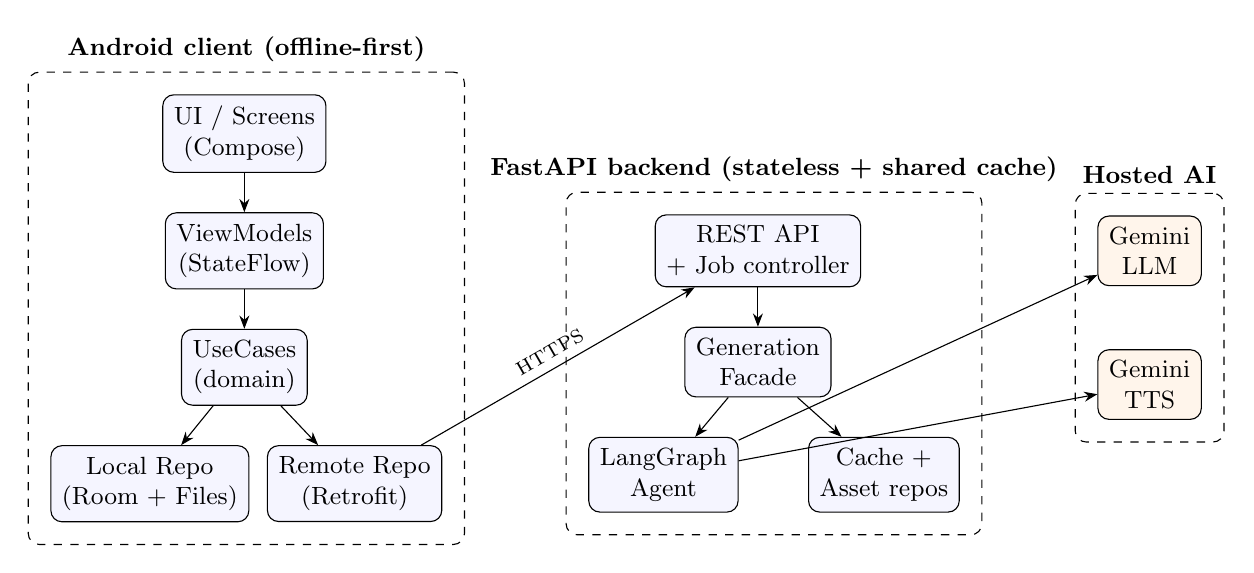
\begin{tikzpicture}[
  font=\small,
  box/.style={draw, rounded corners, align=center, minimum height=8mm,
              inner sep=4pt, fill=blue!4},
  ext/.style={draw, rounded corners, align=center, minimum height=8mm,
              inner sep=4pt, fill=orange!8},
  grp/.style={draw, dashed, rounded corners, inner sep=8pt},
  >={Stealth}
]
% Client column
\node[box] (ui)   {UI / Screens\\(Compose)};
\node[box, below=5mm of ui]   (vm)  {ViewModels\\(StateFlow)};
\node[box, below=5mm of vm]   (uc)  {UseCases\\(domain)};
\node[box, below=5mm of uc, xshift=-12mm] (local) {Local Repo\\(Room + Files)};
\node[box, below=5mm of uc, xshift=14mm]  (remote){Remote Repo\\(Retrofit)};

\begin{scope}[on background layer]
\node[grp, fit=(ui)(vm)(uc)(local)(remote), label=above:{\textbf{Android client (offline-first)}}] (client) {};
\end{scope}

% Backend column
\node[box, right=42mm of vm] (rest) {REST API\\+ Job controller};
\node[box, below=5mm of rest] (facade) {Generation\\Facade};
\node[box, below=5mm of facade, xshift=-12mm] (graph) {LangGraph\\Agent};
\node[box, below=5mm of facade, xshift=16mm]  (cache) {Cache +\\Asset repos};

\begin{scope}[on background layer]
\node[grp, fit=(rest)(facade)(graph)(cache), label=above:{\textbf{FastAPI backend (stateless + shared cache)}}] (backend) {};
\end{scope}

% External column
\node[ext, right=30mm of rest] (llm) {Gemini\\LLM};
\node[ext, below=8mm of llm] (tts) {Gemini\\TTS};

\begin{scope}[on background layer]
\node[grp, fit=(llm)(tts), label=above:{\textbf{Hosted AI}}] (ai) {};
\end{scope}

% edges
\draw[->] (ui) -- (vm);
\draw[->] (vm) -- (uc);
\draw[->] (uc) -- (local);
\draw[->] (uc) -- (remote);
\draw[->] (remote) -- node[above, sloped, font=\scriptsize]{HTTPS} (rest);
\draw[->] (rest) -- (facade);
\draw[->] (facade) -- (graph);
\draw[->] (facade) -- (cache);
\draw[->] (graph) -- (llm);
\draw[->] (graph) -- (tts);
\end{tikzpicture}
\caption{System architecture. A thin offline-first Android client talks to a
stateless FastAPI backend over HTTPS. The backend orchestrates hosted AI through
swappable provider adapters and serves repeated topics from a shared cache.}
\label{fig:arch}
\end{figure*}

\subsection{Key Decisions}
Three decisions shape everything else.

\textbf{Synchronization by pre-rendered timed segments.} Rather than align voice
to highlight at play time, the server splits the narration into segments,
renders one audio clip per segment, and measures each clip's duration. The
device simply plays clips in order and highlights the parts named by the current
clip. This makes synchronization deterministic and removes any need for the
network during playback.

\textbf{Stateless backend with a shared cache.} There are no user accounts on the
server. Lessons are cached by a normalized topic key, so a popular topic is
generated once and then served to everyone. This is cheaper and faster, and it
keeps the server simple to scale and reason about.

\textbf{Provider adapters.} The model and the speech engine sit behind narrow
interfaces. The pipeline talks to those interfaces, never to a vendor SDK
directly. Choosing a model, or replacing the whole vendor, is a configuration
change.

%==============================================================================
\section{Backend Implementation}
\label{sec:backend}
%==============================================================================

The backend is a Python FastAPI application of roughly two thousand lines,
organized by responsibility: an API layer, a domain layer of typed entities and
schemas, provider adapters, the agent graph, services, and repositories. A
single composition root wires these together, which means swapping an
implementation happens in one place plus the typed settings object.

\subsection{Configuration over Hard-Coding}
Everything that varies between environments is read from environment variables
through one typed settings object, following the twelve-factor configuration
guideline~\cite{twelvefactor}. This includes the choice of LLM and TTS provider,
the generation engine, the model identifiers, the storage backend, and the tuning
knobs for the loops. Two points are worth stressing. First, model identifiers are
treated as configuration, not code, because hosted model names change over time;
a small helper lists the live models so the pinned name can be confirmed. At the
time of writing the backend is pinned to a Flash-class Gemini text model (for
example \texttt{gemini-2.5-flash}) and a Flash-class Gemini speech model, both set
in settings rather than in code. Second, the same code base runs on cheap mock
providers or on real Gemini providers depending only on settings, which is what
keeps tests fast and key-free.

\subsection{Provider Adapters}
Two interfaces define what the pipeline needs: an LLM provider that can plan
concepts, draw an SVG, critique and refine an SVG, write narration as structured
data, and repair a drawing-plus-narration given a list of errors; and a TTS
provider that turns text into an audio clip and reports its duration. There are
two implementations of each. The mock implementations are deterministic and need
no network, which makes them ideal for tests and for local development. The
Gemini implementations call the hosted models. The TTS adapter receives raw PCM
audio, wraps it as a WAV file, and computes the exact duration from the byte
count and sample rate, so the duration is a measured fact rather than an
estimate. The adapters also retry transient errors with exponential backoff. A
factory builds a matching set of providers from the settings, following the
abstract factory pattern.

\subsection{The Generation Pipeline}
The heart of the backend is the LangGraph state graph. A single typed state
object flows through the nodes. Figure~\ref{fig:pipeline} shows the graph. The
nodes are as follows.

\begin{figure}[t]
\centering
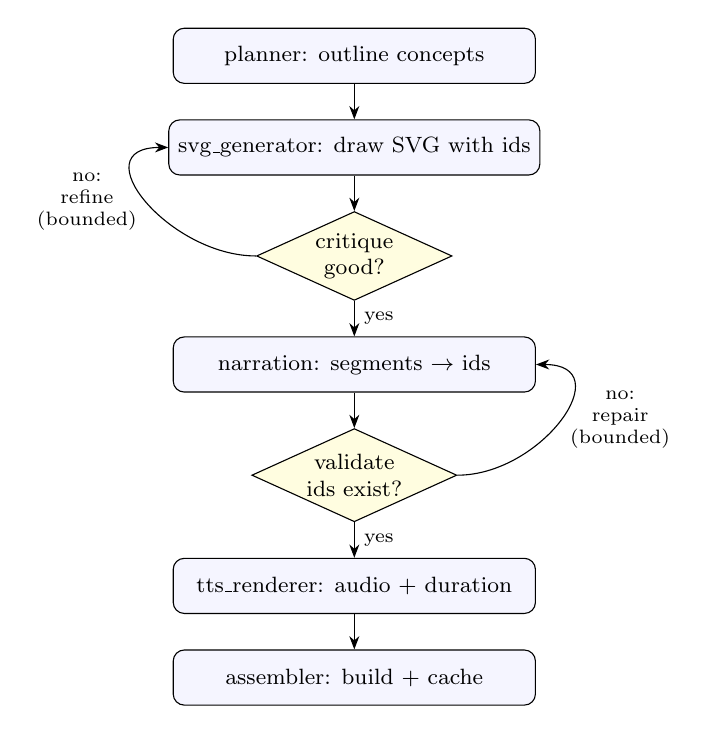
\begin{tikzpicture}[
  font=\footnotesize,
  node distance=4.5mm,
  n/.style={draw, rounded corners, align=center, minimum width=46mm,
            minimum height=7mm, fill=blue!4},
  d/.style={draw, diamond, aspect=2.2, align=center, inner sep=1pt,
            fill=yellow!12},
  >={Stealth}
]
\node[n] (plan) {planner: outline concepts};
\node[n, below=of plan] (svg) {svg\_generator: draw SVG with ids};
\node[d, below=of svg] (crit) {critique\\good?};
\node[n, below=of crit] (narr) {narration: segments $\rightarrow$ ids};
\node[d, below=of narr] (val) {validate\\ids exist?};
\node[n, below=of val] (tts) {tts\_renderer: audio + duration};
\node[n, below=of tts] (asm) {assembler: build + cache};

\draw[->] (plan) -- (svg);
\draw[->] (svg) -- (crit);
\draw[->] (crit) -- node[right,font=\scriptsize]{yes} (narr);
\draw[->] (narr) -- (val);
\draw[->] (val) -- node[right,font=\scriptsize]{yes} (tts);
\draw[->] (tts) -- (asm);

% refine loop (left side)
\draw[->] (crit.west) to[out=180,in=180,looseness=1.6]
  node[left,font=\scriptsize,align=center]{no:\\refine\\(bounded)} (svg.west);
% repair loop (right side)
\draw[->] (val.east) to[out=0,in=0,looseness=1.6]
  node[right,font=\scriptsize,align=center]{no:\\repair\\(bounded)} (narr.east);
\end{tikzpicture}
\caption{The generation graph. A bounded critique-and-refine loop improves the
drawing before narration is written; a bounded repair loop fixes narration that
fails the deterministic validator. A lesson reaches the assembler only after it
passes validation.}
\label{fig:pipeline}
\end{figure}

\emph{Planner.} The model outlines the concepts and a visual plan for the topic.
Planning once, up front, keeps the drawing and the narration aligned to the same
set of concepts.

\emph{SVG generator.} Given the plan, the model draws the SVG and assigns a
semantic \texttt{id} to every meaningful part, for example \texttt{sun},
\texttt{leaf}, and \texttt{chloroplast}.

\emph{Critique and refine.} A critique step scores the drawing and lists
concrete problems. If the score is below a threshold and budget remains, a refine
step redraws with that feedback, then the critique runs again. This loop is
capped by a configurable number of passes. If the budget runs out, the best
drawing so far is accepted and the pipeline moves on. This is a focused use of
the self-critique idea from the literature, applied only to the part that
benefits most.

\emph{Narration generator.} Given the finished drawing, the model writes ordered
narration as structured data: each segment has text and a list of part names. By
writing narration \emph{against} the real drawing, the model is steered toward
referencing parts that exist.

\emph{Validator.} This node uses no model. It parses the SVG as XML, confirms it
is well-formed and has a \texttt{viewBox}, collects the real part names, and
checks that every part name referenced by every segment exists. It also rejects
empty narration and empty segment text. The result is a simple pass-or-fail with
a list of errors.

\emph{Repair.} If validation fails and retries remain, the repair step is given
the exact list of offending names and parse errors and is asked for the minimal
correction, then validation runs again. The loop is bounded; if it is exhausted,
the job fails cleanly rather than caching a broken lesson.

\emph{Renderer.} For each segment, the TTS provider synthesizes audio, the clip
is stored as an asset, and its measured duration is recorded.

\emph{Assembler.} A builder assembles the lesson incrementally: the title, the
SVG and its stored asset, and each segment with its text, part names, audio
asset, and duration. The finished lesson is then cached.

\subsection{The Deterministic Gate}
The validator deserves emphasis because it is the reason the feature is
trustworthy. A model is probabilistic, but the invariant we depend on is binary:
either every referenced part exists or it does not. By enforcing that invariant
in plain, testable code and refusing to cache anything that fails it, we convert
an unreliable generator into a dependable source of lessons. The repair loop is
the bridge: it gives the model a few bounded chances to satisfy the invariant
before we give up. This is the practical answer to the hallucination risk noted
in the related work.

\subsection{Caching, Jobs, and Coalescing}
Because a cold generation can take several seconds, the generate endpoint is
asynchronous. A topic is normalized into a key. On a cache hit the manifest is
returned at once. On a miss a job is created and the client polls a status
endpoint that reports a stage and a percentage until the job reaches a terminal
state. Jobs are keyed by the topic key, so two devices asking for the same topic
at the same time share one job and one generation. The error responses share one
envelope with a code, a message, a retryable flag, and a request identifier, so
the client can react consistently. The result that the client downloads is a
\emph{manifest}, the wire and storage contract for a lesson.
Listing~\ref{lst:manifest} shows its shape.

\begin{lstlisting}[style=json, caption={The lesson manifest (abridged). Audio is
always a downloadable asset; the SVG may be inlined or referenced.},
label={lst:manifest}]
{
  "id": "les_8f3a...",
  "topic": "Photosynthesis",
  "title": "How Photosynthesis Works",
  "language": "en", "voice": "Kore",
  "total_duration_ms": 41200,
  "svg": { "asset_id": "ast_svg_01",
           "url": ".../assets/ast_svg_01" },
  "segments": [
    { "index": 0,
      "text": "Sunlight strikes the leaf...",
      "svg_element_ids": ["sun", "leaf"],
      "audio": { "asset_id": "ast_aud_00",
                 "url": ".../assets/ast_aud_00" },
      "duration_ms": 4200 }
  ]
}
\end{lstlisting}

\subsection{Persistence}
The storage layer is also behind interfaces. A lesson repository hides the
lesson cache and an asset repository hides the object store. In development both
can run in memory or on the local filesystem; the same interfaces allow a
promotion to a database and a cloud object store without touching call sites.
This keeps the dev profile light while leaving a clear path to a production
profile.

%==============================================================================
\section{Client Implementation}
\label{sec:client}
%==============================================================================

The Android client is a Kotlin application of roughly four thousand lines, built
with Jetpack Compose for the user interface and organized with Clean
Architecture and MVVM. The presentation layer holds the screens and view models.
The domain layer holds pure entities, use cases, and repository interfaces with
no Android dependencies. The data layer implements those interfaces with a
Retrofit client for the network, a Room database for metadata, and a file store
for binary assets. Dependencies point inward, so the domain does not know about
the framework. We wire dependencies with a small manual container rather than a
framework, a pragmatic choice that traded a little boilerplate for build
simplicity. Figure~\ref{fig:screens} shows the running app: topic entry, the
synchronized player, and the offline library.

\begin{figure*}[t]
\centering
\begin{minipage}[t]{0.30\textwidth}\centering
  \shot[height=82mm]{fig/home.png}\\[2pt]
  {\footnotesize (a) Topic entry on the home screen}
\end{minipage}\hfill
\begin{minipage}[t]{0.30\textwidth}\centering
  \shot[height=82mm]{fig/player.png}\\[2pt]
  {\footnotesize (b) Player: segment 1 of 6, diagram highlighted}
\end{minipage}\hfill
\begin{minipage}[t]{0.30\textwidth}\centering
  \shot[height=82mm]{fig/library.png}\\[2pt]
  {\footnotesize (c) Offline library of saved lessons}
\end{minipage}
\caption{TutorAI running on a phone. (a) The user types any topic. (b) The
generated lesson plays segment by segment; the diagram parts named by the current
segment are highlighted while its audio plays. (c) Saved lessons replay fully
offline, with no network.}
\label{fig:screens}
\end{figure*}

\subsection{Generation Flow on the Device}
The topic screen takes the typed topic and calls the repository, which performs
the asynchronous job dance: it posts the topic, then polls the job until the
lesson is ready, surfacing progress to the view model as a state flow. The
screen renders that state. When the lesson is ready the user can play it and,
optionally, save it for offline use.

\subsection{Synchronized Playback}
The player is where the product idea becomes visible. The SVG is rendered inside
a WebView as inline markup, with two small JavaScript functions to highlight and
to clear a set of part names. Highlighting is a CSS effect, a glow and a slight
scale, applied to the elements whose identifiers match. The audio is played with
ExoPlayer as a playlist, one media item per segment. The index of the currently
playing clip drives the highlight: when the player advances to clip $k$, the
WebView highlights the part names of segment $k$. Because each clip's start and
end define the highlight window, synchronization is exact and needs no
word-level timing. Figure~\ref{fig:sync} shows this relationship. The transport
controls map onto a small state machine with states for idle, loading, ready,
playing, paused, seeking, and completed. Seeking simply stops the current clip,
clears the highlight, and starts the chosen segment.

\begin{figure}[t]
\centering
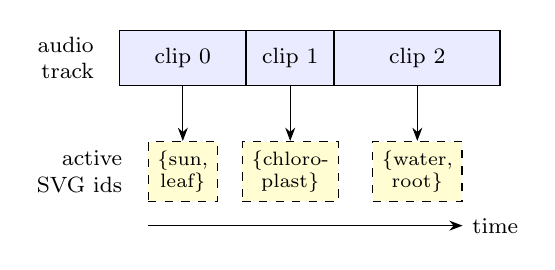
\begin{tikzpicture}[font=\footnotesize, >={Stealth}]
  % audio clips, widths roughly proportional to clip duration
  \node[draw, minimum height=7mm, minimum width=16mm, fill=blue!8] (s0) {clip 0};
  \node[draw, minimum height=7mm, minimum width=11mm, fill=blue!8, right=0pt of s0] (s1) {clip 1};
  \node[draw, minimum height=7mm, minimum width=21mm, fill=blue!8, right=0pt of s1] (s2) {clip 2};
  \node[left=2mm of s0, align=right] {audio\\track};
  % highlighted ids active during each clip
  \node[draw, dashed, below=7mm of s0, fill=yellow!18, align=center, font=\scriptsize] (h0) {\{sun,\\leaf\}};
  \node[draw, dashed, below=7mm of s1, fill=yellow!18, align=center, font=\scriptsize] (h1) {\{chloro-\\plast\}};
  \node[draw, dashed, below=7mm of s2, fill=yellow!18, align=center, font=\scriptsize] (h2) {\{water,\\root\}};
  \node[left=2mm of h0, align=right] {active\\SVG ids};
  \draw[->] (s0.south) -- (h0.north);
  \draw[->] (s1.south) -- (h1.north);
  \draw[->] (s2.south) -- (h2.north);
  % time axis under the highlight boxes
  \draw[->] ([yshift=-3mm]h0.south west) -- ([yshift=-3mm]h2.south east)
    node[right]{time};
\end{tikzpicture}
\caption{Segment-level synchronization. Each audio clip's start and end define
the window during which that segment's SVG element ids are highlighted, so the
picture and the voice stay aligned with no word-level timing and no network.}
\label{fig:sync}
\end{figure}

\subsection{Offline and History}
Saving a lesson downloads the SVG and every audio clip into app-private files
and writes the lesson and its segments into Room. The player is deliberately
source-agnostic: it loads its assets through a lambda, so a saved lesson loads
from local file paths instead of network URLs and replays with no network at
all. The history screen reads from Room, newest first, and supports deletion,
which removes both the database rows and the files. Because there are no
accounts and history is purely local, the privacy goal is met by construction.

%==============================================================================
\section{Engineering for Reliability and Reproducibility}
\label{sec:engineering}
%==============================================================================

A research prototype that only runs on its author's laptop is hard to trust or
extend. We therefore put real effort into the engineering around the system.

\subsection{Design Patterns}
The code uses a small set of well-known patterns~\cite{gamma1994}, each for a
concrete reason, summarized in Table~\ref{tab:patterns}. The patterns are not
used for their own sake; they are the seams that make the system testable and
swappable. The provider interfaces, for instance, are the single point at which
the mock and Gemini implementations differ, which is exactly what lets the test
suite stay key-free while the same code runs against live models in production.

\begin{table}[t]
\caption{Design patterns and why each is used}
\label{tab:patterns}
\centering
\renewcommand{\arraystretch}{1.25}
\begin{tabular}{@{}p{1.7cm}p{5.5cm}@{}}
\toprule
\textbf{Pattern} & \textbf{Purpose in TutorAI} \\
\midrule
Strategy & \texttt{LLMProvider} / \texttt{TTSProvider} interfaces; swap vendor without touching the graph \\
Abstract Factory & build a matching provider set from configuration \\
Adapter & wrap vendor SDKs behind our own interfaces \\
Builder & assemble a valid \texttt{Lesson} incrementally \\
Repository & hide the lesson cache and the asset store \\
Facade & one entry point over cache-check, graph, and persist \\
Pipeline + repair & staged generation with bounded loops (LangGraph) \\
\bottomrule
\end{tabular}
\end{table}

\subsection{Hermetic, Key-Free Testing}
The backend test suite contains forty-eight tests that cover the validator, the
provider factory, the filesystem repository, the graph end to end including both
the repair-recovery and the exhausted-retries paths, the lessons API, audio
handling, and the Gemini adapters. The Gemini adapters are tested against a faked
SDK client, so the suite never calls the live API and never needs a key. A
session fixture disables environment loading and strips the application's
environment variables, which makes the suite hermetic: it produces the same
result on any machine and in continuous integration, with zero external calls.
This is what lets the agent design be exercised cheaply and often. The Android
side uses the repository interfaces as test seams in the same spirit.

\subsection{Containerization and Continuous Delivery}
The backend ships as a container with a health endpoint. Continuous integration
runs the test suite and a container build sanity check on every change to the
backend, and builds a debug application package on every change to the client.
The delivery pipeline builds the backend image, pushes it to a container
registry, and deploys it to a cloud host with a reverse proxy that obtains and
renews a TLS certificate automatically, so the client always talks to the server
over HTTPS with no cleartext exception. A separate workflow builds a signed
release application package when a version tag is pushed and attaches it to a
release. Path filters mean backend changes only trigger backend jobs and client
changes only trigger client jobs. Together these give a reproducible path from a
commit to a running, secured service and an installable application.

%==============================================================================
\section{Implementation Status and Verification}
\label{sec:eval}
%==============================================================================

This is an implementation paper, so we report what the running system produces
and what we verified, and we are explicit about what we have not yet measured.

\textbf{End-to-end generation.} With the real Gemini providers configured, the
pipeline produced a complete lesson for the topic \emph{Photosynthesis}, shown in
Fig.~\ref{fig:diagram}: six narration segments totaling about forty-three seconds
of audio, a well-formed SVG whose parts carry semantic names such as \texttt{sun},
\texttt{leaf}, and \texttt{chloroplast}, narration whose references all passed the
deterministic validator, and real spoken audio for each segment. This exercises
every node of the graph against live models. The saved library in
Fig.~\ref{fig:screens}(c) holds further lessons generated for unrelated
topics---the Pythagorean theorem and Transformer architecture---so the pipeline is
not tuned to a single subject.

\begin{figure}[t]
\centering
\shot[width=\columnwidth]{fig/diagram.png}
\caption{The diagram generated for \emph{Photosynthesis}, as shown in the app's
full-screen view. Each labelled part---the sun, the leaf, the chloroplast, the
water and carbon-dioxide inputs, and the glucose and oxygen outputs---is a
separate SVG element with a stable id, which is exactly what lets the narration
highlight it during playback.}
\label{fig:diagram}
\end{figure}

\textbf{The gate works in both directions.} The graph tests confirm both that a
lesson with a deliberately broken part reference is rejected and routed into the
repair loop, and that when repair cannot fix the problem within the retry budget
the job fails cleanly instead of caching a broken lesson. This is the behavior
the design promises.

\textbf{Reproducibility.} The full suite of forty-eight backend tests passes with
zero live API calls. The container builds and serves its health endpoint, and a
mock-provider generation request returns the expected asynchronous response with
no key present. The client builds an installable package, and the player and
offline paths build against the Room and WebView integrations.

\textbf{What we have not measured.} We have not yet run a formal user study on
learning outcomes, nor a large quantitative study of diagram quality across many
topics, nor on-device latency and battery measurements across a fleet of phones.
We report the system and its verified behavior, and we flag these studies as
future work rather than claiming results we did not collect.
Table~\ref{tab:summary} summarizes the realized system.

\begin{table}[t]
\caption{Realized system at a glance}
\label{tab:summary}
\centering
\renewcommand{\arraystretch}{1.2}
\begin{tabular}{@{}ll@{}}
\toprule
\textbf{Aspect} & \textbf{Realization} \\
\midrule
Backend & FastAPI, $\approx$2.0k LoC Python \\
Client & Android/Compose, $\approx$3.8k LoC Kotlin \\
Generation & LangGraph: plan $\to$ draw $\to$ critique/ \\
           & refine $\to$ narrate $\to$ validate $\to$ repair \\
Gate & deterministic non-LLM validator \\
Models & text + speech via swappable adapters \\
Caching & stateless, topic-keyed, coalesced jobs \\
Offline & Room + file store; network-free replay \\
Tests & 48 hermetic, key-free backend tests \\
Delivery & container + CI/CD + auto-HTTPS \\
\bottomrule
\end{tabular}
\end{table}

%==============================================================================
\section{Discussion and Limitations}
\label{sec:discussion}
%==============================================================================

Several limitations are worth naming plainly.

\emph{Diagram quality has a ceiling.} A language model drawing SVG is good at
clear, well-known concepts and weaker at dense or unusual ones. The
critique-and-refine loop raises the floor but does not guarantee a beautiful
result. The deterministic gate guarantees \emph{consistency}, not aesthetic
quality; a valid lesson can still be a plain one.

\emph{Synchronization is at the segment level.} We light up a group of parts for
a whole sentence, not each part as its word is spoken. This was a deliberate
choice for determinism and offline play. Word-level highlighting would be more
precise but would reintroduce timing data and fragility.

\emph{Cost and latency for cold topics.} The first request for a new topic pays
for several model calls and the speech synthesis, and takes seconds. The shared
cache hides this for repeated topics, and bounded loops cap the worst case, but
the cold path is inherently the slow path.

\emph{Security of generated markup.} Rendering model-produced SVG in a WebView
means the markup must be treated as untrusted. We restrict the WebView to our own
highlight script and avoid executing content-supplied script, but this is an area
that deserves ongoing care.

\emph{Evaluation breadth.} As noted, our claims are about the system's behavior,
not about measured learning gains. A controlled study comparing TutorAI lessons
against static diagrams and against plain text is the most important next step.

%==============================================================================
\section{Conclusion and Future Work}
\label{sec:conclusion}
%==============================================================================

We presented TutorAI, a system that turns a typed topic into a short,
self-explaining lesson: a named vector diagram, segment-level narration tied to
those names, and per-segment audio that drives synchronized highlighting on the
device, fully offline. The core insight is architectural rather than about any
single model. By splitting generation into a small graph of steps, adding a
bounded critique-and-refine loop for the drawing and a bounded repair loop for
the narration, and putting a deterministic, non-LLM validator in front of the
cache, we make a probabilistic generator reliable enough to power a feature that
depends on exact part-to-word correspondence. Around this core, a stateless
caching backend keeps cost down, swappable adapters keep the vendor choice soft,
and an offline-first client keeps the lesson usable without a network. Hermetic
tests, containerization, and continuous delivery make the whole thing
reproducible.

Future work falls into three groups. First, evaluation: a controlled learning
study, a larger automatic study of diagram quality across many topics, and
on-device latency and energy measurements. Second, capability: optional
word-level highlighting where timing allows, richer diagram styles, a research
or planning step in front of the drawing for harder topics, and multi-language
lessons. Third, scale: promoting the in-process worker and filesystem store to a
separate worker, a database, and a cloud object store behind the same interfaces.
None of these change the central design; they extend it.

%==============================================================================
% ACKNOWLEDGEMENT (incl. AI-assistance disclosure per IEEE authorship policy)
%==============================================================================
\section*{Acknowledgment}
The authors used a large language model--based AI assistant (Anthropic's
Claude) to assist in drafting and editing the text of this manuscript. The
system described in this paper---its conception, design, implementation, and
the verification reported---is the authors' own work. The authors reviewed
all text and take full responsibility for the content of this paper.

%==============================================================================
% NOTE: references are listed in order of first appearance, per IEEE style.
\begin{thebibliography}{00}

\bibitem{ji2023hallucination} Z.~Ji \emph{et al.}, ``Survey of hallucination in
natural language generation,'' \emph{ACM Computing Surveys}, vol.~55, no.~12,
pp.~1--38, 2023.

\bibitem{langgraph} LangChain, ``LangGraph: Building stateful, multi-actor
applications with LLMs,'' software documentation. [Online]. Available:
\url{https://langchain-ai.github.io/langgraph/}

\bibitem{bloom1984} B.~S. Bloom, ``The 2 sigma problem: The search for methods
of group instruction as effective as one-to-one tutoring,'' \emph{Educational
Researcher}, vol.~13, no.~6, pp.~4--16, 1984.

\bibitem{anderson1995cognitive} J.~R. Anderson, A.~T. Corbett, K.~R. Koedinger,
and R.~Pelletier, ``Cognitive tutors: Lessons learned,'' \emph{The Journal of
the Learning Sciences}, vol.~4, no.~2, pp.~167--207, 1995.

\bibitem{vanlehn2011} K.~VanLehn, ``The relative effectiveness of human
tutoring, intelligent tutoring systems, and other tutoring systems,''
\emph{Educational Psychologist}, vol.~46, no.~4, pp.~197--221, 2011.

\bibitem{kasneci2023chatgpt} E.~Kasneci \emph{et al.}, ``ChatGPT for good? On
opportunities and challenges of large language models for education,''
\emph{Learning and Individual Differences}, vol.~103, 102274, 2023.

\bibitem{paivio1991} A.~Paivio, ``Dual coding theory: Retrospect and current
status,'' \emph{Canadian Journal of Psychology}, vol.~45, no.~3, pp.~255--287,
1991.

\bibitem{sweller1988} J.~Sweller, ``Cognitive load during problem solving:
Effects on learning,'' \emph{Cognitive Science}, vol.~12, no.~2, pp.~257--285,
1988.

\bibitem{mayer2014multimedia} R.~E. Mayer, Ed., \emph{The Cambridge Handbook of
Multimedia Learning}, 2nd~ed. Cambridge, U.K.: Cambridge Univ. Press, 2014.

\bibitem{mayermoreno2003} R.~E. Mayer and R.~Moreno, ``Nine ways to reduce
cognitive load in multimedia learning,'' \emph{Educational Psychologist},
vol.~38, no.~1, pp.~43--52, 2003.

\bibitem{vaswani2017attention} A.~Vaswani \emph{et al.}, ``Attention is all you
need,'' in \emph{Proc. Advances in Neural Information Processing Systems
(NeurIPS)}, 2017, pp.~5998--6008.

\bibitem{brown2020gpt3} T.~B. Brown \emph{et al.}, ``Language models are
few-shot learners,'' in \emph{Proc. Advances in Neural Information Processing
Systems (NeurIPS)}, 2020, pp.~1877--1901.

\bibitem{gemini2023} Gemini Team, Google, ``Gemini: A family of highly capable
multimodal models,'' arXiv:2312.11805, 2023.

\bibitem{wei2022cot} J.~Wei \emph{et al.}, ``Chain-of-thought prompting elicits
reasoning in large language models,'' in \emph{Proc. Advances in Neural
Information Processing Systems (NeurIPS)}, 2022.

\bibitem{yao2023react} S.~Yao \emph{et al.}, ``ReAct: Synergizing reasoning and
acting in language models,'' in \emph{Proc. Int. Conf. Learning Representations
(ICLR)}, 2023.

\bibitem{madaan2023selfrefine} A.~Madaan \emph{et al.}, ``Self-Refine: Iterative
refinement with self-feedback,'' in \emph{Proc. Advances in Neural Information
Processing Systems (NeurIPS)}, 2023.

\bibitem{shinn2023reflexion} N.~Shinn \emph{et al.}, ``Reflexion: Language
agents with verbal reinforcement learning,'' in \emph{Proc. Advances in Neural
Information Processing Systems (NeurIPS)}, 2023.

\bibitem{chen2023selfdebug} X.~Chen, M.~Lin, N.~Sch\"arli, and D.~Zhou,
``Teaching large language models to self-debug,'' arXiv:2304.05128, 2023.

\bibitem{langchain} H.~Chase, ``LangChain,'' open-source software, 2022.
[Online]. Available: \url{https://github.com/langchain-ai/langchain}

\bibitem{liu2023promptsurvey} P.~Liu \emph{et al.}, ``Pre-train, prompt, and
predict: A systematic survey of prompting methods in natural language
processing,'' \emph{ACM Computing Surveys}, vol.~55, no.~9, pp.~1--35, 2023.

\bibitem{rombach2022stable} R.~Rombach, A.~Blattmann, D.~Lorenz, P.~Esser, and
B.~Ommer, ``High-resolution image synthesis with latent diffusion models,'' in
\emph{Proc. IEEE/CVF Conf. Computer Vision and Pattern Recognition (CVPR)},
2022, pp.~10684--10695.

\bibitem{svgspec} World Wide Web Consortium (W3C), ``Scalable Vector Graphics
(SVG) 1.1 (Second Edition),'' W3C Recommendation, 2011. [Online]. Available:
\url{https://www.w3.org/TR/SVG11/}

\bibitem{carlier2020deepsvg} A.~Carlier, M.~Danelljan, A.~Alahi, and
R.~Timofte, ``DeepSVG: A hierarchical generative network for vector graphics
animation,'' in \emph{Proc. Advances in Neural Information Processing Systems
(NeurIPS)}, 2020.

\bibitem{rodriguez2023starvector} J.~A. Rodriguez \emph{et al.}, ``StarVector:
Generating scalable vector graphics code from images,'' arXiv:2312.11556, 2023.

\bibitem{chen2021codex} M.~Chen \emph{et al.}, ``Evaluating large language
models trained on code,'' arXiv:2107.03374, 2021.

\bibitem{oord2016wavenet} A.~van den Oord \emph{et al.}, ``WaveNet: A generative
model for raw audio,'' arXiv:1609.03499, 2016.

\bibitem{shen2018tacotron2} J.~Shen \emph{et al.}, ``Natural TTS synthesis by
conditioning WaveNet on mel spectrogram predictions,'' in \emph{Proc. IEEE Int.
Conf. Acoustics, Speech and Signal Processing (ICASSP)}, 2018, pp.~4779--4783.

\bibitem{offlinefirst} A.~Feyerke, ``Designing offline-first web apps,'' \emph{A
List Apart}, no.~373, 2013. [Online]. Available:
\url{https://alistapart.com/article/offline-first/}

\bibitem{androidguide} Google, ``Guide to app architecture,'' Android Developers
documentation. [Online]. Available:
\url{https://developer.android.com/topic/architecture}

\bibitem{martin2017clean} R.~C. Martin, \emph{Clean Architecture: A Craftsman's
Guide to Software Structure and Design}. Boston, MA: Prentice Hall, 2017.

\bibitem{twelvefactor} A.~Wiggins, ``The Twelve-Factor App,'' 2017. [Online].
Available: \url{https://12factor.net/}

\bibitem{gamma1994} E.~Gamma, R.~Helm, R.~Johnson, and J.~Vlissides,
\emph{Design Patterns: Elements of Reusable Object-Oriented Software}. Reading,
MA: Addison-Wesley, 1994.

\end{thebibliography}

\end{document}
